% Generated from floating-point data (illustration only; not used in any proof).
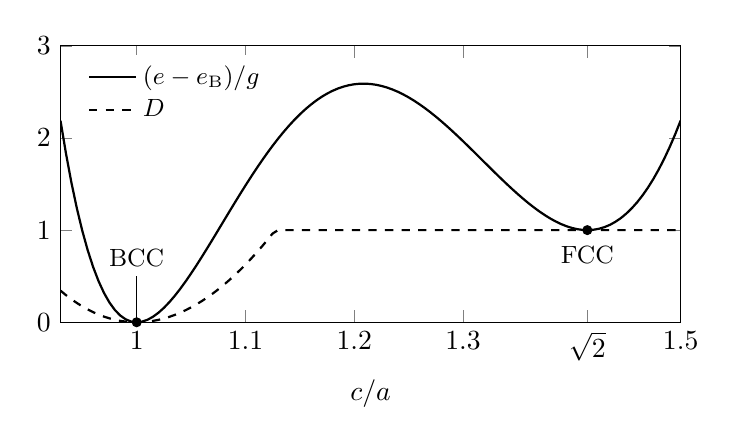
\begin{tikzpicture}
\begin{axis}[width=0.78\textwidth,height=0.42\textwidth,xmin=0.93,xmax=1.5,ymin=0,ymax=3,
  xlabel={$c/a$},ylabel={},xtick={1,1.1,1.2,1.3,1.4142,1.5},xticklabels={$1$,$1.1$,$1.2$,$1.3$,$\sqrt2$,$1.5$},
  ytick={0,1,2,3},legend pos=north west,legend cell align=left,legend style={draw=none,font=\small}]
\addplot[thick,black] coordinates {
(0.930,2.1877) (0.935,1.8328) (0.940,1.5171) (0.945,1.2382) (0.950,0.9938) (0.955,0.7816) (0.960,0.5995) (0.965,0.4455) (0.970,0.3176) (0.975,0.2140) (0.980,0.1328) (0.985,0.0725) (0.990,0.0312) (0.995,0.0076) (1.000,0.0000) (1.005,0.0071) (1.010,0.0275) (1.015,0.0600) (1.020,0.1033) (1.025,0.1563) (1.030,0.2178) (1.035,0.2868) (1.040,0.3623) (1.045,0.4435) (1.050,0.5293) (1.055,0.6189) (1.060,0.7117) (1.065,0.8067) (1.070,0.9034) (1.075,1.0011) (1.080,1.0992) (1.085,1.1970) (1.090,1.2941) (1.095,1.3900) (1.100,1.4842) (1.105,1.5763) (1.110,1.6659) (1.115,1.7526) (1.120,1.8361) (1.125,1.9162) (1.130,1.9926) (1.135,2.0649) (1.140,2.1331) (1.145,2.1970) (1.150,2.2563) (1.155,2.3109) (1.160,2.3608) (1.165,2.4059) (1.170,2.4461) (1.175,2.4813) (1.180,2.5115) (1.185,2.5367) (1.190,2.5570) (1.195,2.5723) (1.200,2.5828) (1.205,2.5884) (1.210,2.5893) (1.215,2.5856) (1.220,2.5773) (1.225,2.5646) (1.230,2.5476) (1.235,2.5265) (1.240,2.5015) (1.245,2.4726) (1.250,2.4402) (1.255,2.4043) (1.260,2.3653) (1.265,2.3232) (1.270,2.2784) (1.275,2.2310) (1.280,2.1813) (1.285,2.1296) (1.290,2.0761) (1.295,2.0210) (1.300,1.9647) (1.305,1.9073) (1.310,1.8492) (1.315,1.7907) (1.320,1.7321) (1.325,1.6736) (1.330,1.6155) (1.335,1.5582) (1.340,1.5019) (1.345,1.4470) (1.350,1.3938) (1.355,1.3425) (1.360,1.2935) (1.365,1.2472) (1.370,1.2038) (1.375,1.1637) (1.380,1.1272) (1.385,1.0946) (1.390,1.0663) (1.395,1.0426) (1.400,1.0237) (1.405,1.0102) (1.410,1.0022) (1.415,1.0001) (1.420,1.0042) (1.425,1.0150) (1.430,1.0326) (1.435,1.0575) (1.440,1.0900) (1.445,1.1303) (1.450,1.1789) (1.455,1.2361) (1.460,1.3022) (1.465,1.3775) (1.470,1.4623) (1.475,1.5570) (1.480,1.6620) (1.485,1.7774) (1.490,1.9037) (1.495,2.0411) (1.500,2.1901)
};
\addlegendentry{$(e-e_{\mathrm B})/g$}
\addplot[thick,black,dashed] coordinates {
(0.930,0.3430) (0.935,0.2947) (0.940,0.2502) (0.945,0.2094) (0.950,0.1725) (0.955,0.1392) (0.960,0.1096) (0.965,0.0836) (0.970,0.0612) (0.975,0.0424) (0.980,0.0270) (0.985,0.0152) (0.990,0.0067) (0.995,0.0017) (1.000,0.0000) (1.005,0.0017) (1.010,0.0066) (1.015,0.0149) (1.020,0.0263) (1.025,0.0410) (1.030,0.0588) (1.035,0.0798) (1.040,0.1039) (1.045,0.1311) (1.050,0.1613) (1.055,0.1946) (1.060,0.2309) (1.065,0.2702) (1.070,0.3123) (1.075,0.3574) (1.080,0.4055) (1.085,0.4563) (1.090,0.5101) (1.095,0.5666) (1.100,0.6259) (1.105,0.6881) (1.110,0.7529) (1.115,0.8205) (1.120,0.8908) (1.125,0.9637) (1.130,1.0000) (1.135,1.0000) (1.140,1.0000) (1.145,1.0000) (1.150,1.0000) (1.155,1.0000) (1.160,1.0000) (1.165,1.0000) (1.170,1.0000) (1.175,1.0000) (1.180,1.0000) (1.185,1.0000) (1.190,1.0000) (1.195,1.0000) (1.200,1.0000) (1.205,1.0000) (1.210,1.0000) (1.215,1.0000) (1.220,1.0000) (1.225,1.0000) (1.230,1.0000) (1.235,1.0000) (1.240,1.0000) (1.245,1.0000) (1.250,1.0000) (1.255,1.0000) (1.260,1.0000) (1.265,1.0000) (1.270,1.0000) (1.275,1.0000) (1.280,1.0000) (1.285,1.0000) (1.290,1.0000) (1.295,1.0000) (1.300,1.0000) (1.305,1.0000) (1.310,1.0000) (1.315,1.0000) (1.320,1.0000) (1.325,1.0000) (1.330,1.0000) (1.335,1.0000) (1.340,1.0000) (1.345,1.0000) (1.350,1.0000) (1.355,1.0000) (1.360,1.0000) (1.365,1.0000) (1.370,1.0000) (1.375,1.0000) (1.380,1.0000) (1.385,1.0000) (1.390,1.0000) (1.395,1.0000) (1.400,1.0000) (1.405,1.0000) (1.410,1.0000) (1.415,1.0000) (1.420,1.0000) (1.425,1.0000) (1.430,1.0000) (1.435,1.0000) (1.440,1.0000) (1.445,1.0000) (1.450,1.0000) (1.455,1.0000) (1.460,1.0000) (1.465,1.0000) (1.470,1.0000) (1.475,1.0000) (1.480,1.0000) (1.485,1.0000) (1.490,1.0000) (1.495,1.0000) (1.500,1.0000)
};
\addlegendentry{$D$}
\addplot[only marks,mark=*,mark size=1.6pt,black] coordinates {(1,0) (1.41421,1)};
\node[anchor=south,font=\small] at (axis cs:1,0.5) {BCC};
\draw[thin] (axis cs:1,0.5) -- (axis cs:1,0.05);
\node[anchor=north,font=\small] at (axis cs:1.41421,0.93) {FCC};
\end{axis}
\end{tikzpicture}
